\chapter{Solution approach}

% ~~~~~~~~~~~~~~~~~~~~~~~~~~~~~~~~~~~~~~~~~~~~~~~~~~~~~~~~~~~~~~~~~~~~~~~~~~~~~~~~~~~~~~~~~~~~~~~~~~~~~~~~~~~
\section{Baseline solution}

\begin{itemize}
    \item Adapt existing simple indicators to detect bottlenecks.
        All the indicators consider the relationship between the processing times of jobs on the machines
        and the total (or idle) time.
        
        This idea is still applicable on the \ac{rcpsp}. However, given that the machine load can be variable
        through time, a binary \enquote{processing-idle} differentiation between machine states does not
        provide a sufficient machine-load indication.

        

    \begin{figure}[ht]
      \centering
      \subfloat[Job Shop]{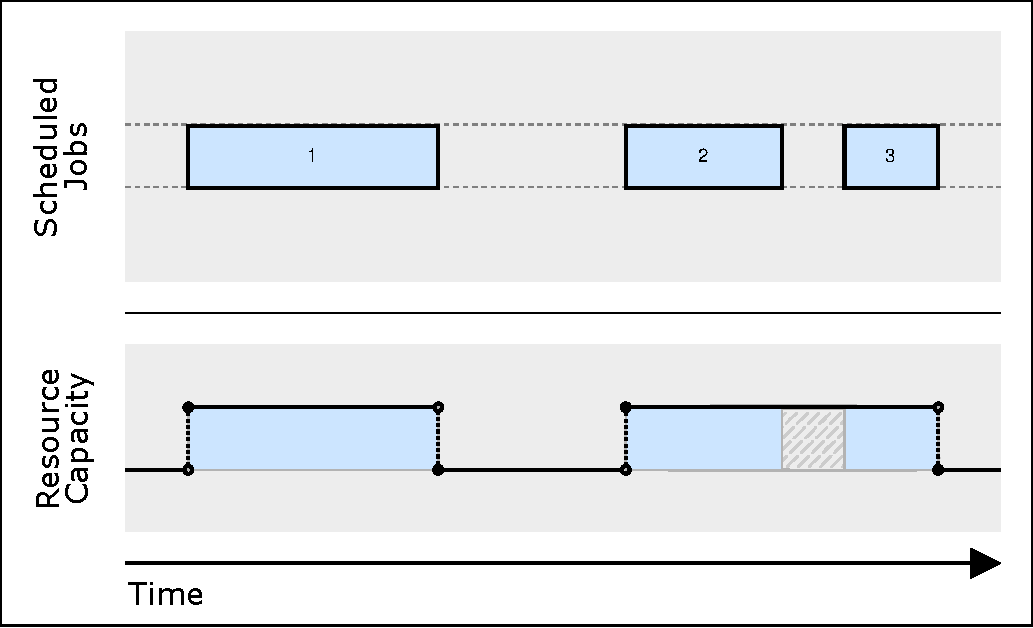
\includegraphics[width=0.45\textwidth]{img/Capacities-JobShop.pdf}\label{fig:f1}}
      \hfill
      \subfloat[RCPSP]{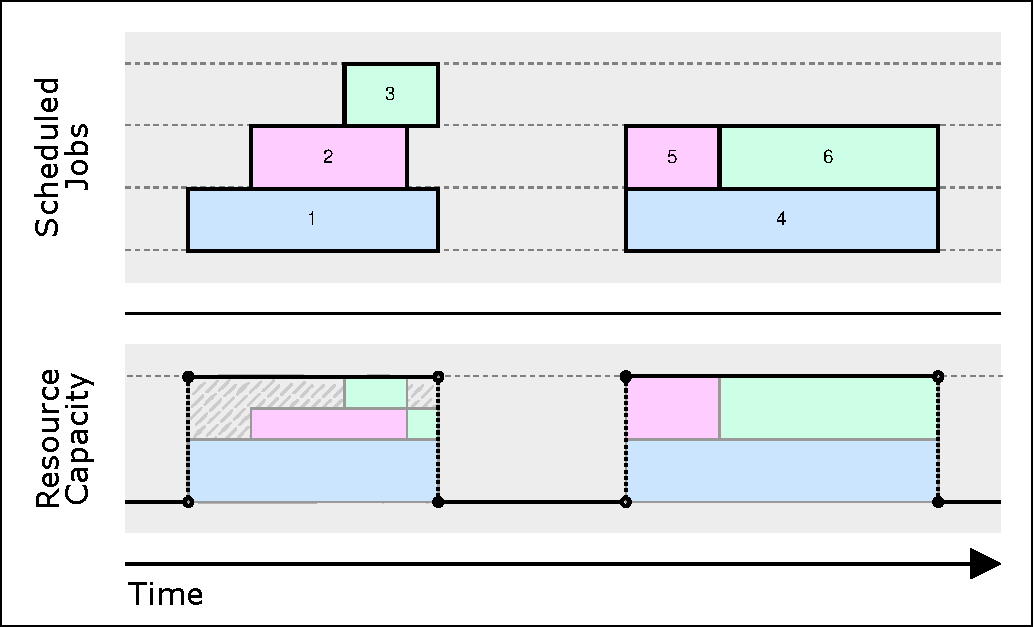
\includegraphics[width=0.45\textwidth]{img/Capacities-RCPSP.pdf}\label{fig:f2}}
      \caption{Caption.}
    \end{figure}
    \begin{itemize}
        \item Machine Workload

        \item Machine Utilization Rate

        \item Average Uninterrupted Active Duration
    \end{itemize}

    \item Try to find alternative schedule based on the found bottlenecks
    \begin{itemize}
        \item Combinatorial heuristics?
        \item Simplified optimization?
    \end{itemize}
\end{itemize}

% ~~~~~~~~~~~~~~~~~~~~~~~~~~~~~~~~~~~~~~~~~~~~~~~~~~~~~~~~~~~~~~~~~~~~~~~~~~~~~~~~~~~~~~~~~~~~~~~~~~~~~~~~~~~
\section{Extended solution}

\begin{itemize}
    \item Come up with a new way of detecting time-variant bottlenecks
    \item Apply the method to identify bottlenecks
    \item Relax bottlenecks - one by one, combined?
    \item Propose alternative solutions
    \begin{itemize}
        \item Extremal solutions based on some similarity/improvement metrics?
        \item Scalable solution?
    \end{itemize}
\end{itemize}
